\chapter{Hadron Interactions in Argon: Cross Section}\label{ch:Interactions}
\section{Literature Review}

%the prediction of the total hadronic interaction cross section ($\pi^{\pm}$, Ar) for thin-target simulations from two Monte Carlo generators (Geant 4.10.1 with Bertini Cascade model~\cite{geant4, g4bert} and Genie v2.8.2 with intranuke-hA model). The thick target simulation used a simple stand-alone Geant4 simulation  (i.e., no other detector features were taken into account except the geometry of the thin slices in the LAr volume). Fig.~\ref{fig:xsplot} shows the resulting total ${\pi^-}$ cross section extracted by the sliced TPC technique; it agrees well with the Geant 4 thin-target cross section. The Genie thin-target cross section for $^{40}$Ar shown in this figure is significantly different than that of Geant at low kinetic energies due to the fact that Geant4 models are tuned on $^{12}$C while Genie ones are tuned on a much heavier $^{56}$Fe target. The extrapolated cross section predicted for $^{40}$Ar can be then very different, especially in the resonance region where the model is strongly target-dependent from one generator to another.
 
%The comparison of the Geant4 thin- and thick-target cross section results demonstrates the power of the "sliced TPC" method for the measurement of the ($\pi^{\pm}$, Ar) cross section in LArIAT TPC geometry. 


%Having validated the ``Sliced TPC'' technique and shown that the this technique recovers the simulated cross-section, we now move to performing this measurement utilizing the complete LArIAT simulation within the LArSoft \cite{} based simulation.  Furthermore, we move from utilizing particle level MC-truth information to performing fully automated reconstruction of the charged hadron events within the LArTPC. 


%Since the kaon cross section in argon has never been measured before, the Geant4 Monte Carlo tunes kaon transportation in argon by extrapolation from lighter and heavier nuclei. As shown in the previous section,  kaon data on carbon are available and  can be used as a metric to evaluate the Geant4 prediction performances.  Figure \ref{fig:TrueCarbon} shows the total hadronic cross section for carbon implemented in Geant4 10.01.p3 overlaid with the Bugg and Friedman data. Unfortunately, the current version of Geant4 does not reproduce the data for carbon closely. On one hand, this evidence makes us even more wary when using the Monte Carlo in simulating the kaon-argon interactions. On the other, it further highlights the importance of kaon measurements.

\section{How to Measure a Hadron Cross Section in LArIAT}\label{ch:methodology}
We use both the LArIAT  beamline detectors and the LArTPC information in order to measure hadronic cross sections in argon. Albeit with small differences, both the  $\pi^{-}$~-~Ar and K$^{+}$~-~Ar total hadronic cross section measurements rely on the same procedure described in details in the following paragraphs: we select the particle of interest using a combination of beamline detectors and TPC information (paragraph \ref{ch:ParticleSelectionMethod}), we perform a handshake between the beamline information and the TPC tracking to assure we are selecting the right TPC track (paragraph \ref{ch:WC2TPCMatchMethod}), and we apply the ``thin slice" method to get to the final result (paragraph \ref{ch:ThinSliceMethod}). We show a cross check of this method in paragraph \ref{ch:procedureTesting}.

\subsection{Event Selection}\label{ch:ParticleSelectionMethod}

\subsubsection{Particle Identification in the beamline}
In data, the main tool used to identify the hadron of interest for the cross section calculation is the LArIAT tertiary beamline, in its function of mass spectrometer. We combine the measurement of the time of flight, $TOF$, and the beamline momentum, $p_{Beam}$, to reconstruct the invariant mass of the particles in the beamline, $m_{Beam}$, as follows
\begin{equation}
m_{Beam} = \frac{p_{Beam}}{c}\sqrt{\biggl(\frac{TOF*c}{l}\biggr)^2 -1},
\end{equation}
 where $c$ is the speed of light and $l$ is the length of the particle trajectory between the time of flight paddels. 

Figure \ref{fig:mass} shows the mass distribution for the Run II negative polarity runs on the left and positive polarity runs on the right. We perform the classification of events into the different samples as follows:

\begin{itemize}
\item \underline{$\pi, \mu, e$:} 0~MeV $<$ mass $<$ 350~MeV

\item \underline{kaon:} 350~MeV $<$ mass $<$ 650~MeV

\item \underline{proton:} 650~MeV $<$ mass $<$ 3000~MeV.

\end{itemize}


%\begin{comment}     
\begin{figure}
%\captionsetup{justification=raggedright}  
\begin{minipage}[b]{.53\textwidth}  
  \centering  
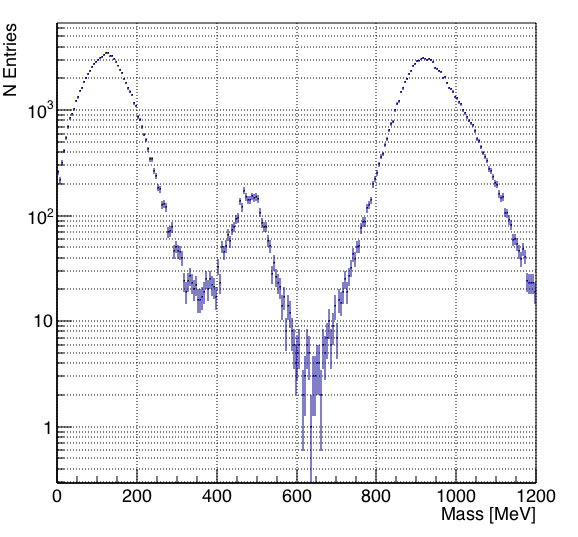
\includegraphics[width=3in]{Chapter-4/Images/massRunIIPos.png}
\end{minipage}%  
\begin{minipage}[b]{0.53\textwidth}  
  \centering  
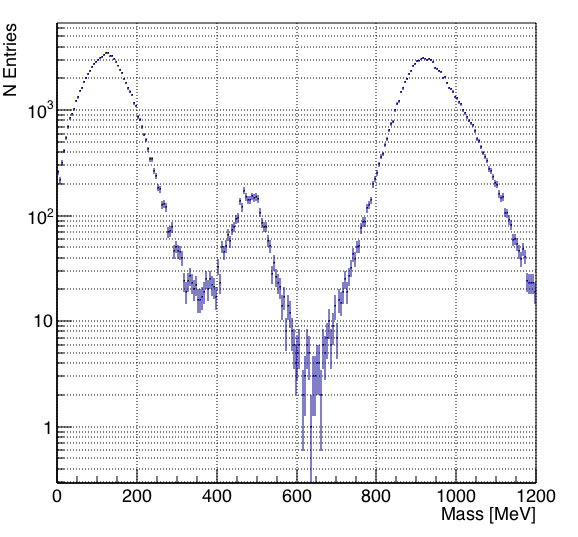
\includegraphics[width=3in]{Chapter-4/Images/massRunIINeg.png}
\end{minipage}
\caption{The mass plotted for a sample of Run-II events reconstructed in the beamline, negative polarity runs on the left and positive polarity runs on the right. The classification of the events into $\pi, \mu, e$, kaon, or proton is based on this distribution.\textcolor{red}{CHANGE PLOTS}}
\label{fig:mass}
\end{figure}

\subsubsection{Additional Particle Identification technique}\label{ch:electrons}
For the $\pi^-$-Ar cross section, the resolution of  beamline mass spectrometer is not sufficient to select a beam of pure pions. In fact, muons and electrons survive the selection on the beamline mass value. It is important to notice that the composition of the negative polarity beam is mostly pions, as discussed in \ref{ch:beamlineComposition}.
Anyhow, we devise a selection on the TPC information to mitigate the presence of electrons in the sample used for the pion cross section. The selection relies on the different topologies of a pion and an electron event in the argon: while the former will trace a track inside the TPC active volume, the latter will tend to ``shower", i.e. interact with the medium, produce bremsstrahlung photons which pair convert into several short tracks. We provide details of this selection in section \ref{ch:electronCuts}.

\subsubsection{Pile up mitigation }\label{ch:pileUp}
The secondary beam impinging on LArIAT secondary target produces a pletora of particles. The number of particle which trace down the LArIAT beamline is greatly abated by the presence of upstream and downstream collimators. 
%because of pile up particles during the triggered TPC drift time

We adjust the primary beam intensity between LArIAT Run I and Run II to minimize the presence of pile up events in the data sample. We remove from the cross section sample events with more than 4 tracks in the first 14 cm upstream portion of the TPC.

\subsection{Wire Chamber to TPC Match}\label{ch:WC2TPCMatchMethod}
If an event passes the selection on its beamline information, we need to identify the track inside the TPC corresponding to the particle which triggered the beamline detectors, a procedure we refer to as ``WC to TPC match" (WC2TPC for short). In general, the TPC tracking algorithm will reconstruct more than one track in the event, partially due to the fact that hadrons interact in the chamber, as shown in figure \ref{fig:pionInteraction}, and partially because of pile up particles during the triggered TPC drift time, as shown in figure \ref{fig:pionPileUp}. 
\textcolor{red}{ADD EVENT DISPLAYS}

In data, we attempt to uniquely match one wire chamber track to one and only one reconstructed TPC track. This match leverages on a geometrical selection on both the position of the wire chamber and TPC tracks and the angle between them. We consider only TPC tracks whose first point is in the first 2 cm upstream portion of the TPC for the match.  We project the wire chamber track to the TPC front face where we define the $x_{FF}$ and $y_{FF}$ coordinates used for evaluating the match.  We define $\Delta$X as the difference between the $x$ position of the most upstream point of the TPC track and $x_{FF}$.  $\Delta$Y is defined analogously. We define the radius difference, $\Delta$R, as $ \Delta \text{R} =  \sqrt{ \Delta \text{X}^2 +  \Delta \text{Y}^2}  $. The angle between the incident WC track and the TPC track in the plane that contains them defines $\alpha$.  If  $\Delta \text{R} < 4 $~cm, $\alpha < 8^\circ $,  a match between WC-track and TPC reconstructed track is found. We describe  how we determinate the best value for the radius and angular selection in sec \ref{ch:WC2TPCMatchOptimization}.
In MC, we mimic the matching between the WC and the TPC track by constructing a fake WC track using truth information at wire chamber four. We then apply the same WC to TPC matching algorithm as in data. 
We discard events with multiple WC2TPC matches. We use only TPC track matched to WC tracks in the cross section calculation.


\subsection{The Thin Slice Method}\label{ch:ThinSliceMethod}
\subsubsection{Cross Sections on Thin Target}
Cross section measurements on a thin target have been the bread and butter of nuclear and particle experimentalists since the Rutherford experiments \textcolor{red}{NEED CITATION}. At their core, this type of experiments consists in shooting a beam of particles with a known flux on a thin target and recording the outgoing flux. 


In general, the target is not a single particle, but rather a slab of material containing many diffusion centers. The so-called  ``thin target" approximation assumes that the target centers are uniformly distributed in the material and that the target is thin compared to the interaction length so that no center of interaction sits in front of another. In this approximation, the ratio between the number of particles interacting in the target $N_{Interacting}$ and number of incident particles $N_{Incident}$ determines the interaction probability $P_{Interacting}$, which is the complementary to one of the survival probability $P_{Survival}$. 
Equation \ref{eq:thinTargetXS} 
\begin{equation}
P_{Survival} = 1- P_{Interacting} = 1 - \frac{N_{Interacting}}{N_{Incident}} = e^{-\sigma_{TOT} n \delta X}
\label{eq:thinTargetXS}
\end{equation}
describes the probability for a particle to survive the thin target. This formula relates the total cross section $\sigma_{TOT}$, the density of the target centers  $n$  and  the thickness of the target  along the incident hadron direction $\delta X$, to the interaction probability\footnote{The scattering center density in the target, {\emph{n}},  relates to the argon density $\rho$, the Avogadro number  $ N_{A} $ and the argon molar mass $m_A$ as $n=\frac{\rho N_{A} }{m_A}$.}. If the target is thin compared to the interaction length of the process considered, we can Taylor expand the exponential function in equation \ref{eq:thinTargetXS} and find a simple proportionality relationship between the number of incident and interacting particles, and the cross section, as shown in equation \ref{eq:thinTargetXSTaylor}:
\begin{equation}
1 - \frac{N_{Interacting}}{N_{Incident}} =  1 -\sigma_{TOT} n \delta X + O(\delta X^2).
\label{eq:thinTargetXSTaylor}
\end{equation}

Solving for the cross section, we find:
\begin{equation}
 \sigma_{TOT}  = \frac{1}{n \delta X}\frac{N_{Interacting}}{N_{Incident}}.
\label{eq:thinTargetXSSolved}
\end{equation}

\subsubsection{Not-so-Thin Target: Slicing the Argon}
The LArIAT TPC, with its 90 cm of length, is not a thin target. \textcolor{red}{Find expected interaction length for hadrons and kaons}. However, the fine-grained tracking of the LArIAT LArTPC allows us to treat the argon volume as a sequence of many adjacent thin targets. 

As described in section \ref{sec:experimentDescription}, LArIAT wire planes count 240 wires each. The wires are oriented at +/- $60^{\circ}$ from the vertical direction at 4 mm spacing, while the beam direction is oriented 3 degrees off the $z$ axis in the $XZ$ plane. \textcolor{red}{review this math} The wires collect signals proportional to the energy loss of the hadron along its path in a  $\delta${\emph{X}} = 4 mm/sin($60^{\circ}$) $\approx$ 4.7~mm slab of liquid argon. Thus, one can think to slice the TPC into many thin targets of $\delta${\emph{X}} = 4.7~mm thickness along the direction of the incident particle. 

Considering each slice {\emph{j}}  a ``thin target",  we can apply the cross section calculation from Eq.~\ref{eq:thinTargetXSSolved} iteratively, evaluating the kinetic energy of the hadron as it enters each slice, $E_{j}^{kin}$.  For each WC-to-TPC matched particle, the energy of the hadron entering the TPC is known thanks to the momentum and mass determination by the tertiary beamline, 

\begin{equation}
 E^{kin}_{Front Face}  = \sqrt{p^2_{Beam} - m^2_{Beam}} - m_{Beam} - E_{loss},
\label{eq:enFF}
\end{equation}
where $E_{loss}$ is a correction for the energy loss in the dead material between the beamline and the TPC front face (more on \ref{sec:Eloss}). The  energy of the hadron at the each slab is determined by subtracting the energy released by the particle in the previous slabs. For example, at the $j^{th}$ point of a track, the kinetic energy will be

\begin{equation}
 E_{j}^{kin} =  E^{kin}_{Front Face} - \sum_{i < j} \Delta E_i,
\label{eq:KEj}
\end{equation}
where $\Delta E_i$ is the energy deposited at each argon slice before the $j^{th}$ point as measured by the calorimetry associated with the tracking.


If the particle enters a slice, it contributes to $N_{Incident}( E^{kin})$ in the energy bin corresponding to its kinetic energy in that slice. If it interacts in the slice, it then also contributes to $N_{Interacting}(E^{kin})$ in the appropriate energy bin. The cross section as a function of kinetic energy, $\sigma_{TOT}( E^{kin})$ will then be proportional to the ratio $\frac{N_{Interacting}( E^{kin})}{N_{Incident}( E^{kin})}$ .


The statistical uncertainty for each energy bin is calculated by error propagation from the statistical  uncertainty on $N_{Incident}$ and $N_{Interacting}$. 
Since the number of incident hadrons in each energy bin is given by a simple counting, we assume that $N_{Incident}$ is distributed as a poissonian with mean and $\sigma^2$ equal to $N_{Incident}$ in each bin.  
On the other hand, $N_{Interacting}$ follows a binomial distribution: a particle in a given energy bin might or might not interact.  The square of the variance for the binomial is given by  
\begin{equation}
\sigma^2 = \mathcal{N}P_{Interacting}(1-P_{Interacting});
\label{eq:binVar}
\end{equation}

since the interaction probability $P_{Interacting}$ is $\frac{ N_{Interacting}}{N_{Incident}}$ and the number of tries $\mathcal{N}$ is $N_{Incident}$, equation \ref{eq:binVar} translates into
\begin{equation}
\sigma^2 = N_{Incident}\frac{ N_{Interacting}}{N_{Incident}} (1-\frac{ N_{Interacting}}{N_{Incident}}) = N_{Interacting}(1-\frac{ N_{Interacting}}{N_{Incident}}).
\end{equation}

$N_{Incident}$ and $N_{Interacting}$ are not independent.
The uncertainty on the cross section is thus calculated as 
\begin{equation}
\delta\sigma_{tot}(E) = \sigma_{tot}(E) \Big(\frac{\delta N_{Interacting}}{N_{Interacting}}+\frac{\delta N_{Incident}}{N_{Incident}}\Big) 
\end{equation}
where:
\begin{eqnarray}
\delta N_{Incident} = \sqrt[]{N_{Incident}} \\
\delta N_{Interacting} = \sqrt[]{N_{Interacting}\Big(1-\frac{ N_{Interacting}}{N_{Incident}}\Big)}.
\end{eqnarray}


%%%%%%%%%%%%%%%%%%%%%%%%%%%%%%%%%%%%%%%%%%%%%%%%



\subsection{Procedure testing with truth quantities}\label{ch:procedureTesting}
The $\pi^{-}$-Ar and K$^{+}$-Ar total hadronic cross section implemented in Geant4 can be used as a tool to validate the measurement methodology.  We describe here a closure test done on Monte Carlo to prove that the methodology of slicing the TPC retrieves the underlying cross section distribution implemented in Geant4 within the statistical error. %under the working assumption of perfect reconstruction.

For pions in the considered energy range, \textcolor{red}{the Geant4 inelastic model adopted to is ``BertiniCascade", while the elastic model ``hElasticLHEP".}
For kaons, the Geant4 inelastic model adopted to is ``BertiniCascade", while the elastic model ``hElasticLHEP".  


For the validation test, we fire about 390000 pions and 140000 kaons inside the LArIAT TPC active volume using the DDMC (see sec \ref{ch:DDMC}). We apply  the thin-sliced method on using true quantities to calculate the hadron kinetic energy at each slab in order to decouple reconstruction effects to eventual issues with the methodology.  For each slab of 4.7 mm length on the path of the hadron, we integrate the true energy deposition as given by the Geant4 transportation model. Then, we recursively subtracted it from the hadron kinetic energy at the TPC front face to evaluate the kinetic energy at each slab until the true interaction point is reached. Doing so, we obtain the true interacting and incident distributions for the considered hadron and we obtain the true MC cross section as a function of the hadron true kinetic energy. 

Figure \ref{fig:TrueMCXS} shows the total hadronic cross section for argon implemented in Geant4 10.01.p3 (solid lines) overlaid with the true MC cross section as obtained with the sliced TPC method (markers) for pions on the left and kaons on the right; the total cross section is shown in green,  the elastic cross section in blue and the inelastic cross section in red.  The nice agreement with the Geant4 distribution and the cross section  obtained with the sliced TPC method gives us confidence in the  validity of the methodology. 
        
%\begin{comment}     
\begin{figure}
%\captionsetup{justification=raggedright}  
\begin{minipage}[b]{.53\textwidth}  
  \centering  
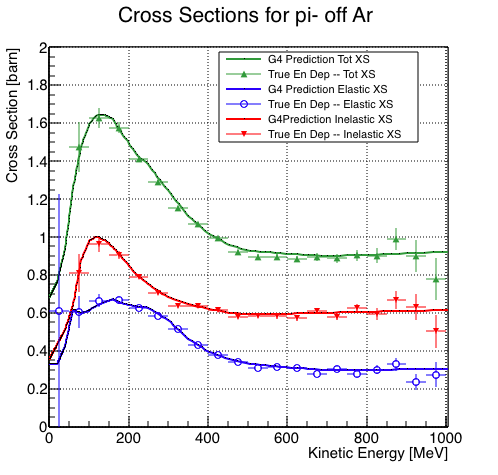
\includegraphics[width=3in]{Chapter-4/Images/PionTrueXS.png}
\end{minipage}%  
\begin{minipage}[b]{0.53\textwidth}  
  \centering  
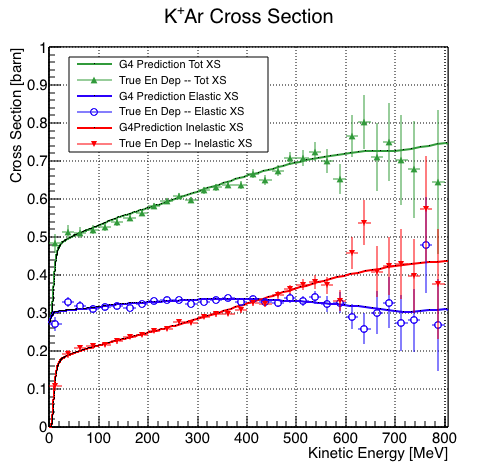
\includegraphics[width=3in]{Chapter-4/Images/KaonTrueXS.png}
\end{minipage}
\label{fig:TrueMCXS}
\caption{Hadronic cross sections for $\pi^-$-Ar (left) and K$^+$-Ar (right) implemented in Geant4 10.01.p3 (solid lines) overlaid the true MC cross section as obtained with the sliced TPC method (markers). The total cross section is shown in green,  the elastic cross section in blue and the inelastic cross section in red.}
%\par
%\begin{minipage}[t]{.53\textwidth}
%\caption{total hadronic cross section for carbon implemented in Geant4  10.01.p3  with overlaid with the Bugg %and Frideman data.}
%\label{fig:TrueCarbon}
%\end{minipage}%
%\begin{minipage}[t]{.5\textwidth}  
%\caption{Hadronic cross sections for argon implemented in Geant4 10.01.p3 (solid lines) overlaid the true MC cross section as obtained with the sliced TPC method (markers). The total cross section is shown in green,  the elastic cross section in blue and the inelastic cross section in red.}
%\label{fig:TrueArgon}
%\end{minipage}  
\end{figure}
%\end{comment}




%%%%%%%%%%%%%%%%%%%%%%%%%%%%%%%%%%%%%%%%%%%%%%%%%
%%%%%%%%%%%%%%%%%%%%%%%%%%%%%%%%%%%%%%%%%%%%%%%%%
%%%%%%%%%%%%%%%%%%%%%%%%%%%%%%%%%%%%%%%%%%%%%%%%%
%%%%%%%%%%%%%%%%%%%%%%%%%%%%%%%%%%%%%%%%%%%%%%%%%


\chapter{Uncertainty budget}
Measuring an hadronic cross section  in LArIAT translates into counting how many hadrons impinged on a slab of argon at a given energy and how many of those hadrons interacted at said energy. So, the key questions here are:
\begin{itemize}
\item[]a) how well do we know the kinetic energy at each point of the tracking? %(Incident Kinetic Energy bins)
\item[]b) how well do we know when the tracking stops? %(Interacting Kinetic Energy bin)
\item[]c) are there any systematic shifts?
\end{itemize}

In order to answer this question, will discuss first a simple scenario  were our beam is 100\% made of pions which arrive as primaries in the TPC (no decay in the beam and no inelastic interaction before the TPC front face). We will then add a layer of complexity by discussing how we handle beamline contamination.

\section{Pure beam of pions}
Assuming a beam of pure pions gets to the TPC, let us explicit some of the variables in the kinetic energy equation \ref{eq:KEj}  to point out the important quantities in the uncertainty budget,

\begin{align}
 E_{j}^{kin} &=  E_{Beam}^{kin}  - E_{loss} - \sum_{i < j} \frac {dE_i}{dx_i}*dx_i\\
                  &=  \sqrt{p^2_{Beam} - m^2_{Beam}} - m_{Beam} - E_{loss} - \sum_{i < j} \frac {dE_i}{dx_i}*dx_i.
\end{align}

\subsection{Uncertainty on $E_{Beam}^{kin}$}
Let us start by discussing the uncertainty on $E_{Beam}^{kin}$. Since we are assuming a beam of pions, the uncertainty on the value of mass of the pion ($m_{Beam}$) as given by the pdg is irrelevant compared to the momentum uncertainties, thus $\delta E_{Beam}^{kin} = \delta p_{Beam}^{kin}$. 
We estimate the momentum uncertainty as follows.

\textcolor{blue}{  
We estimate the uncertainty on a 4-point track. In case of 3-points track, we add an additional 2\% coming from Greg's study. 
Uncertainty on a 4-point track:
\begin{itemize}
\item[-]  Alignment surveys. 1mm misalignment translates to 3\% in overall
\item[-] Doug study dp/p = ~2\% based on field map (docdb 1710)
\item[-] Minerva test beam paper
\end{itemize}
}

\subsection{Uncertainty on $E_{loss}$}
We estimate the uncertainty on the energy loss between the beamline momentum measurement and the TPC, $E_{loss}$, using the DDMC pion sample. We shoot pions from WC4 with the same momentum distribution as in the beamline data and plot the true $E_{loss}$ for that sample. The width of the $E_{loss}$ distribution is the $\delta E_{loss}$.

\textcolor{blue}{ TO DO HERE: make sure we have the geometry right, cause otherwise this correction is meaningless.  With this method, so far we get a mean ~40 MeV, but uncertainty ~7MeV. 
The trajectory method does not improve uncertainty, why? It's a mystery I don't think we should solve before June :) .
Back of the envelope material budget calculation:}
\begin{table}[h!]
\centering
\caption{Back of the envelope calculation}
\label{my-label}
\begin{tabular}{|l|l|l|l|}
\hline
dEdx for MIP, MPV {[}MeV cm$^2$/gr{]} & density {[}g/cm$^3${]} & width {[}cm{]} & E$_{loss}$ {[}MeV{]} \\ \hline
1.6                                                 & 1.7 (G10)                            & 1.3            & 3.5                   \\
1.6                                                 & 1.4 (LAr)                            & 1.77           & 4.0                   \\
1.6                                                 & 7.7 (S.S.)                           & 0.23           & 2.8                   \\
1.6                                                 & 4.5 (Ti)                             & 0.04           & 0.3                   \\ 
1.6                                                 & 1.03 (Plastic Sci)                   & 1.1            & 1.8                   \\ \hline
Total                                               &                                      &                & 12.4                  \\ \hline
\end{tabular}
\end{table}


\textcolor{blue}{Event taking into account a 3 degree bent, we get 12.41 MeV, which is quite far from 40 MeV... something smells here ;)}

\subsection{Uncertainty on dE/dx and pitch}
We obtain the uncertainty on dE/dx and track pitch by comparing the dE/dx and pitch distributions in data and MC.
\textcolor{blue}{ Currently, MPV MC = 1.70 and MPV DATA = 1.72 MeV/cm (~3\% higher).
TO DO HERE: calculate Argon density from mid-RTD temperature. Compare this  density with MC Argon density. 
Density change  affects dE/dx (in MeV/cm!). Try changing MC density up to ``real one" and see if dEdX agrees between DATA and MC}


\subsection{Uncertainty on track end, aka efficiency correction}
From the MC, we obtain an efficiency correction on the interacting and incident distributions separately. This is done by comparing the MC reconstructed with the true MC deposition on an event by event basis.
This correction is applied bin by bin on the data interacting and incident distributions.
The better our tracking, the smaller this efficiency correction will be. So, step number one is improving the tracking.
\textcolor{blue}{Need to talk to Bruce about this.}
\textcolor{blue}{ I don't understand the angle cut that Dave Schmitz and Jon Paley were so vocal about.}

Now, the key question remains: does the tracking behave in the same way in data and MC? 
We can compare some key plots between reconstructed data and MC which gives us confidence this is true: the track pitch, the tracks straightness and the goodness of fit in data and MC. \textcolor{blue}{ Does such a variable as ``goodness of fit" exists in the tracking? We should ask Bruce.}

\section{Handling beamline contamination}
What is the beamline contamination? We define beamline contamination every TPC track matched to the WC track which is not a primary pion. There are 4 different types of beamline contaminations:
\begin{itemize}
\item[]1) electrons,
\item[]2) muons,
\item[]3) secondaries from pion events,
\item[]4) matched pile up events.
\end{itemize}

So, how do we handle this contamination?

The first step is to estimate what percentage of events used in the cross section calculation is not a primary pion.  
We estimate the percentage of electrons and muons in the beam via the beamline MC\footnote{Since the beamline composition is a function of the magnet settings, we simulate separately events for magnet current of -60A and -100A. 
We calculate the electron to pion and muon to pion ratio on the whole sample as the weighted sum of the corresponding ratio in the two current settings, 
\begin{equation}
\frac{N_e}{N_\pi}_{Data} = w_{60A}\frac{N_e}{N_\pi}_{60A}  + w_{100A}\frac{N_e}{N_\pi}_{100A},
\end{equation}
\begin{equation}
\frac{N_\mu}{N_\pi}_{Data} = w_{60A}\frac{N_\mu}{N_\pi}_{60A}  + w_{100A}\frac{N_\mu}{N_\pi}_{100A},
\end{equation}
where the weights $w_{60A}$ and $w_{100A}$ are the percentage of events in the corresponding magnet configuration passing the mass selection in data. }.
Once the beam composition is know,  we simulate the electrons, muons and pions with the DDMC and we subject the three samples to the same selection chain (WC2TPC match, shower filter, pile up filter, etc...). The percentage of electrons and muons surviving the selection chain is the  electron and muon contamination in the pion cross section sample.
The percentage of secondaries is given in the MC by the number of matched WC2TPC tracks which are not flagged as primary by Geant4.
We estimate the last type of contamination, the ``matched pile up" events, to be a negligible fraction, because of the definition of the WC2TPC match: we deem the probability of a single match with a halo particle in the absence of a beamline particle\footnote{ Events with multiple WC2TPC matches are always rejected.} extremely small.


Once we estimate the contaminants to primary pion ratio, the next step is subtracting their contribution from data for each type of contaminant independently. The contaminant samples are reconstructed and the corresponding interacting and incident histograms are produced. We then perform a bin by bin subtraction in the data interacting and incident histograms separately. A graphical rendering of this procedure is shown in Fig \ref{fig:backgroundSubtraction}
Once the data is background subtracted, we apply the correction laid out in the previous section.
\textcolor{blue}{How do we account for the error in the contamination subtraction? We change the electron/pion and muon/pion ratio and we see how much difference we get?}

\begin{figure}
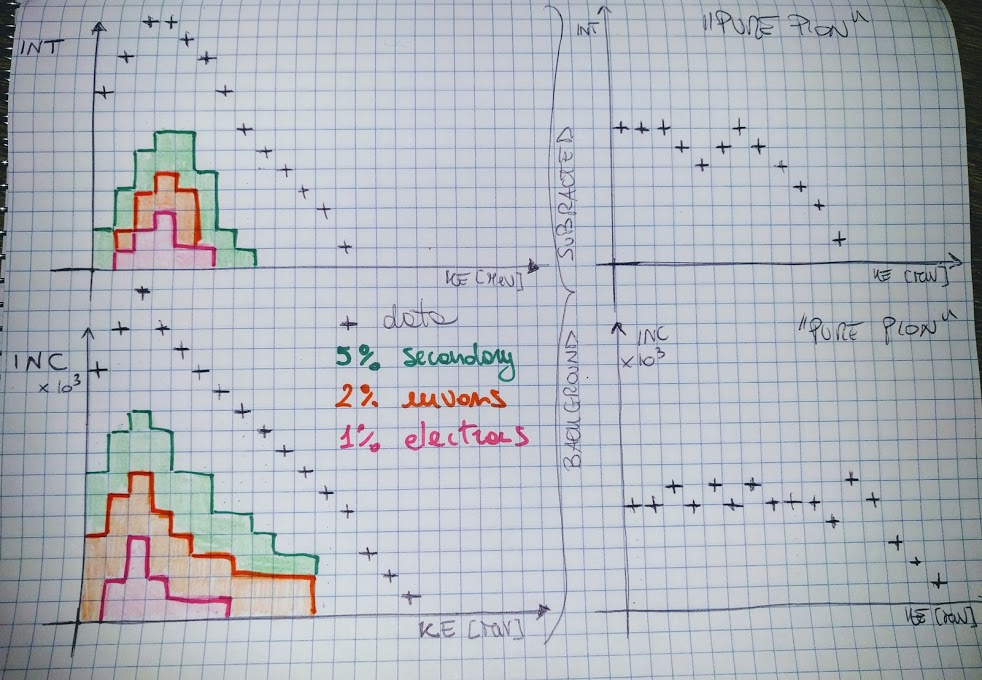
\includegraphics[width=\textwidth,height=\textheight,keepaspectratio]{Chapter-4/Images/FakePlot.jpg}
\label{fig:backgroundSubtraction}
\caption{A graphical rendering of the beamline contamination background subtraction. The contribution of the contaminants is shown in green for the secondaries, in orange for the muons and in pink for electrons. The colored plots are coming from the MC and are staggered. The percentages shown in the legend are the percentages of contaminants over the total number of events  passing the selection chain. We actually expect way less contamination.}
\end{figure}



